% cJASguide.tex
% v4.4 released October 2008

\documentclass[useAMS]{cJAS2e}

%%%%%%%%%%%%%%%%%%%%%  monte adds %%%%%%%%%%%%%%%
%\usepackage{lscape}
\usepackage{pdflscape}
\usepackage{multirow}
\usepackage{tabularx,tabulary}
\usepackage{arydshln}

\usepackage{subfig}  % subfloat
\usepackage{units}  %% nicefrac

\usepackage{undertilde}  %% \undertilde{} and \tilde{}  %% under and over
\newcommand{\undertilde}[1]{\utilde{#1}}


\DeclareGraphicsExtensions{.png}
\usepackage{moreverb}
\usepackage{verbatim}

\def\inprob{\,{\buildrel p \over \longrightarrow}\,}
\def\eqdist{\,{\buildrel d \over =}\,}
\def\indist{\,{\buildrel d \over \longrightarrow}\,}
\def\eqdist{\,{\buildrel d \over =}\,}
\def\isDist{\,{\buildrel {\ } \over \sim}\,}
\def\IIDdist{\,{\buildrel iid \over \sim}\,}
\def\iseq{\,{\buildrel ? \over =}\,}
\def\asymdist{\,{\buildrel a \over \sim}\,}
\def\approxdist{\,{\buildrel \cdot \over \sim}\,}

\usepackage{setspace}
\usepackage{fancyhdr}
\usepackage{lastpage}
\usepackage{extramarks}
\usepackage{chngpage}
\usepackage{soul,color}
\usepackage{graphicx,float,wrapfig}
\usepackage{todonotes}

% \todo[color=green!40]{And a green note}
% http://www.tex.ac.uk/CTAN/macros/latex/contrib/todonotes/todonotes.pdf

\definecolor{gray}{rgb}{0.5,0.5,0.5}

\newcommand{\added}[1]{\textcolor{blue}{#1}}
\newcommand{\changed}[1]{\textcolor{red}{#1}}
\newcommand{\removed}[1]{\textcolor{gray}{#1}}

\newcommand{\reviewer}[1]{\todo[color=green!40, size=\tiny]{#1}}

%%%%%%%%%%%%%%%%%%%%%%%%%%%%%%%%%%%%%%%%%%%%%%%%%%%%%%%%%%%%%%%%%%%%%%%%%%%%%%%%%%%%%%%%%%%%%%%%%%%%%%%%%%%%%%%%%

\begin{document}
\doi{10.1080/0266476YYxxxxxxxx}
\issn{1360-0532}
\issnp{0233-1934}
\jvol{00} \jnum{00} \jyear{2011} \jmonth{February}
\publisher{Dasgupta and Shaffer}

\markboth{Nairanjana Dasgupta and Monte J. Shaffer}{Journal of Applied Statistics}




\articletype{RESEARCH ARTICLE}

\title{Many-to-one Comparison of Nonlinear Growth Curves for Washington's Red Delicious Apple}

\author{Nairanjana Dasgupta$^{\rm a}$$^{\ast}$\thanks{$^\ast$Corresponding author. Email: dasgupta@wsu.edu
\vspace{6pt}} and Monte J. Shaffer$^{\rm b}$\\\vspace{6pt}  $^{\rm a}${\em{Professor, Department of Statistics, Washington State University, Pullman WA, 99164-3144}}; $^{\rm b}${\em{Postdoctoral Research Fellow,  McGuire Center for Entrepreneurship, University of Arizona, Tucson AZ 85721-0108}}\\\vspace{6pt}\received{January 2012 [rev. 1]} }



\maketitle

\begin{abstract}
In this article we are interested in comparing growth curves for the red delicious apple in several locations to that of a reference site.  Although such multiple comparisons are common for linear models, statistical techniques for nonlinear models are not prolific.  We theoretically derive a test statistic considering the issues of sample size and design points. Under equal sample sizes and same design points our test statistic is based on the  maximum of an equi-correlated multivariate chi-square distribution.  Under unequal sample sizes and design points we derive a general correlation structure, and then utilize the multivariate normal distribution to numerically compute critical points for the maximum of the multivariate chi-square.  We apply this statistical technique to compare the growth of Red Delicious apples \changed{at six locations to a reference site} in the state of Washington in 2009.  Finally, we perform simulations to verify the performance of our proposed procedure for Type I error and marginal power.  Our proposed method performs well in regard to both.

\bigskip

\begin{keywords}multiple comparisons to control; multivariate chi-square distribution; nonlinear growth curves; Richard's curve; simulated critical points
\end{keywords}\bigskip

\end{abstract}


\section{Introduction}\label{sec:intro}
The state of Washington is a leading agricultural state and grows over half of the apples produced in the U.S. annually. Of all the apples it produces, Washington is most recognized for its Red Delicious apple.  It is one of the big export crops for the state of Washington.  It has long been of interest of growers and horticulturists to understand the growth pattern of apples.  As a result, the Washington Tree Fruit Commission is collecting data over the next three years to model the growth of Washington's Red Delicious apple.  The data set used in this manuscript was collected between May and August 2009.  The data were collected at a reference \reviewer{\textbf{(R3: \P \ 1)} In the footnote, we briefly discuss the choice of Naches as the referent.} site\footnote{\added {Naches is a small, agrarian town where large quantities of tree-fruit are commercially grown:  mostly apples, pears, cherries, and peaches.  Naches is located in central Washington in the heart of Yakima valley, along the Naches River (a tributary of the Columbia River).  Working with the Washington Tree Fruit Research, we chose Naches as the reference site during the design of the experiment.  Based on this choice, appropriate resources were allocated to the Naches site enabling more frequent (see Table \ref{tbl:results-1}) apple-growth observations. }} (Naches) and six other research stations across the state (Omak, Chelan, Orondo, Wenatchee, Royal City, Wapato), see Figure~\ref{fig-wa-apples}.  One of the initial questions asked was: is there a difference in the growth pattern for the six sites to that of the reference site?



%This will allow the Commission to plan out strategies for data collection over the next two years.

\begin{figure}[h!]		
		\begin{center}	
    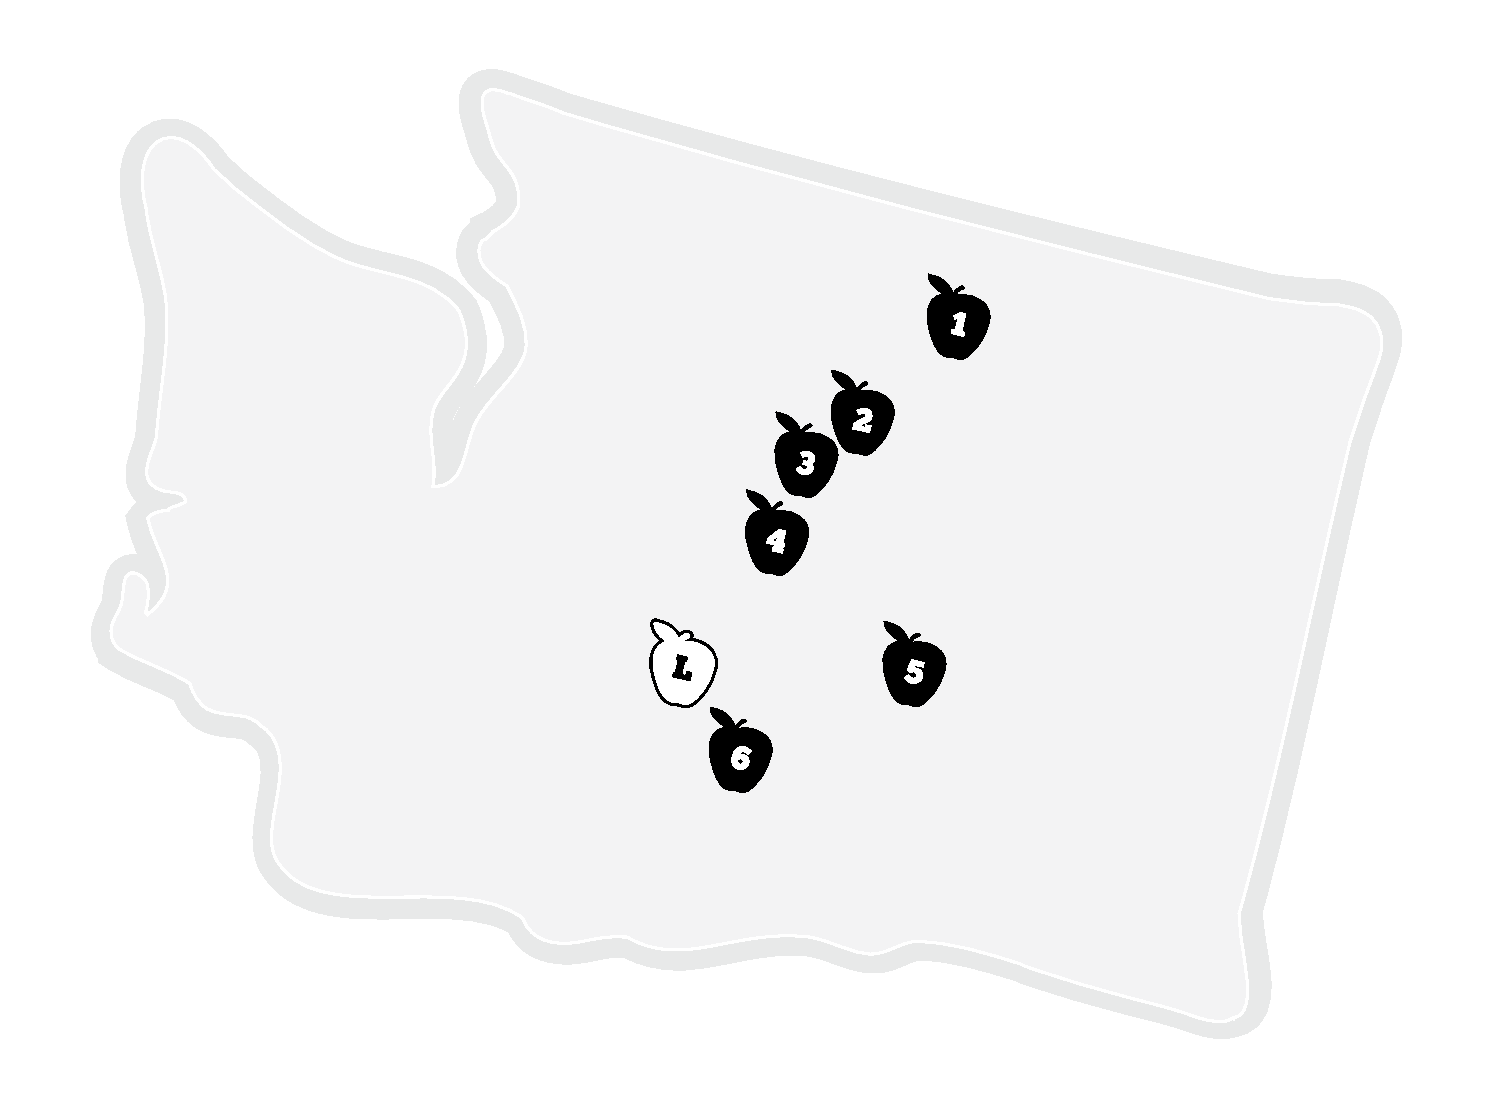
\includegraphics[width=0.8\textwidth]{graphics/AppleMap_trim.pdf}
  \end{center}
  \caption{\textbf{Multiple comparison of growth}:  Are there differences in growth patterns at the six research stations (labeled 1-6) compared to the reference cite (labeled L)?}
  \label{fig-wa-apples}
\end{figure}

 Apple growth has been studied extensively using several different units of analysis and many different types of models.  Studies in photosynthesis \citep{Blanke:1992}, the root stock \citep{Abbott:1960,Zeller:1991,Pawlicki:1995,Kelner:2000}, the tree growth itself \citep{Seems:1986}, the fruit load on tree architecture \citep{Kelner:2000,Costes:2006}, and the entire orchard system \citep{Hester:2003} all relate to the final output of apple sizes and yields \citep{Welte:1990}.   There have been temperature studies \citep{Johnson:1986} relating to the importance of rest \citep{Champagnat:1989,Cook:2005}, blossoming \citep{Fulford:1966a,Fulford:1966b} of fruit buds \citep{Landsberg:1974} with early-season temperatures \citep{Austin:1999}, and other temperature measures \citep{Tromp:1994}.  Understanding final sizes and yields are complicated because there are so many different ways to model the growth of the apple, and depending on the practices at a given orchard, there may be variability in outcomes.

Our data comprises of repeated diameter measurements from bloom to harvest for a sample of Red Delicious apples at the seven different locations. \changed{Research has shown that this} diameter depends on cell count, volume, and density \citep{Coombe:1976,Wu:1999}.  Diameter growth, in general, has been described as a sigmoidal or double sigmoid growth curve \citep{Lakso:1995}.

\section{Statistical precedence}\label{sec:sbg}
The study of growth in the biological sciences is the foundation of mathematical statistics.  From the studies of crop variation by R.A. Fisher \citep*{Fisher:1963}, to the human characteristic studies of Karl Pearson \citep{Pearson:1902,Pearson:1906}, most statistical techniques have been developed to understand and study growth. Early work on growth curves was very descriptive in nature focusing on cross-tabular comparisons of key variables such as age, gender, and height on weight \citep{Hacker:1944}.   Potthoff \citet{Potthoff:1964} developed a generalized multivariate analysis of variance (MANOVA) model to solve basic ``Growth Curve Problems" including tests to compare the growth of two groups (males and females) using ``m"-parameter polynomial models and the expectation of the growth outcome(s).  This generalized form has been demonstrated to be very robust \citep{Potthoff:1964,Rao:1965,Lee:1974,Baksalary:1978,Verbyla:1986,Verbyla:1988,Fujikoshi:1991}, and relies on F-tests to determine the order of the polynomial to consider and to compare an unrestricted effects-model (e.g., gender effect, could be multivariate) to a restricted model (all parameters are equal to some common vector of parameters).  Such analysis addresses fundamental aspects of multiple comparison \citep{ONeill:1971,Einot:1975,Hsu:1996}; however, there is a need for more sophisticated multiple comparison techniques to compare groups simultaneously.

The literature comparing growth curves is not as prolific.  Royen \citet{Royen:1984} discussed a method for comparing several polynomials. Heckman and Zemar \citet{Heckman:2000} describe a nonparametric technique that address shapes and groups simultaneously.  Dasgupta et al. \citet{Dasgupta:2000} focus on comparing several logistic regression curves.  Another heuristic multiple-comparison approach has been developed by Bretz et al. \citet{Bretz:2005}.  They describe a technique to search among various generalized models (mostly nonlinear) to identify a best model that explains optimal dosages across treatments while controlling for ``family-wise error rates"  using critical values simulated from a multivariate \emph{t} distribution \citep{Genz:2004}.


% Finally, we offer a numeric computation to define critical points for an unequal design frame.

\section{Our contribution}\label{sec:our}
In this article, we introduce a general multiple comparison technique for nonlinear models.  Specific to the study of apple growth, we apply this technique to a three-parameter  \changed{variation of the nonlinear model} known as the Richards' Curve \citep{Richards:1959}, yet we derive a test statistic that can be applied to any $k$-parameter nonlinear model.  Similary, we emphasize that we apply this technique specifically to compare 6 locations to a reference site; however, this technique can be applied to any $L-1$ multiple comparisons (locations, treatments, etc.) to a referent.  Additionally, we provide methods of calculating the test statistic based on the number of \changed{actual observations at any particular site}.  In the real world, the execution of a design is not always ideal, as circumstances prevent simultaneous measurement, apples fall off the tree, etc.  Our approach accounts for such a reality.



\section{Model Specification}\label{sec:growth}

Many sigmoid growth functions are available to model apple growth.  In this research, we \changed{choose to utilize} a three-parameter \added{variation} of the  Richards' Curve \citep{Richards:1959} to model apple growth: 

\begin{equation}\label{eqn:richards3-location}
	Y_{ji} = f(X_{ji};\undertilde{\Theta}_{i}) = f(X_{ji};\beta_i,\delta_i,\tau_i) = \frac{\beta_i}{\left(1 +  e^{- \delta_i (X_{ji}-\tau_i)} \right)}
\end{equation}

\noindent where $Y_{ji}$ represents the growth of the \changed{apple's ($j$)} diameter (in inches) for location $i$ at time $X_{ji}$.



Generally, the nonlinear model is fit using various observations at specific points in time ($X_{ji}$) for a given location.  For example, 100 apples may be measured at 6 different points in time to give a total sample size of 600 observations for a specific location.  Another location, however, may sample 100 apples measured at 9 design points, and these 9 points may or may not be different that the 6 design points for the first location.  We describe this phenomenon in this form $X_{n_j,s}$ where $n_j$ is the number of observations at a given design point and $s$ is the number of design points.  From this, the number of observations for a location is defined as $N_i = \sum_{j=1}^s n_j$.  The last two columns of Table \ref{tbl:results-1} describes details regarding the design points (Julian days when data are collected)  and number of fruit collected at each site.


\added{We choose \reviewer{\textbf{(R1: \P \ 4-5)} In the paragraph, we briefly discuss our model selection, the parameters of this model, and nonlinearity issues.} this model for several reasons.  First, the parameters have conceptual meaning to the apple growers:  the maximum apple size ($\beta$), its growth rate ($\delta$), and the time of maximum growth ($\tau$).  Second, this three-parameter model assumes: that at time $X_{ji}=0$ the apple's size is zero;  growth is symmetric around its inflection point ($X_{ji}=\tau_i$); the carrying capacity represents the maximum apple size; and this model form would allow for accomodating other factors by including more parameter .  Third, this specific variation of the Richard's curve is a reasonably-behaved\footnote{\added{Ratkowsky \citet{Ratkowsky:1990} defines the full Richard's model parameterization as a ``particular unfortunate model because not only is its parameter-effects (PE) nonlinearity high but so too is its intrinsic (IN) nonlinearity" due to its overgenerality (see p. 47).  The three-parameter variation we chose is defined to be ``one of the most versatile and useful models" as this symmetric model having good estimation properties of $\tau$ and a finite upper asymptote (see 5.3.2 on p. 128).}  } nonlinear model.}  

\changed{Based on our model selection, the} parameter vector $\Theta$ for each location $i$ is

\begin{equation}\label{eqn:params3-location}
\undertilde{\Theta}_{i} = \left( \begin{array}{c} {\beta}_i \\  {\delta}_i \\ {\tau}_i \end{array} \right),
\end{equation}

\noindent which defines a $k=3$ parameter model; 



\added{We estimate our parameter vector using the Gauss-Newton method \reviewer{\textbf{(R1: \P \ 4-5)} In the paragraph, we briefly discuss the method to estimate the nonlinear model.} to get our Least Square estimate vector for each location as $\undertilde{\hat{\Theta}}_{i}$.  We define the $\text{var}(\undertilde{\hat{\Theta}}_{i}) = \Sigma_i$.  The form of $\Sigma_i$ depends upon the method\footnote{\added{These estimates have desirable properties, in the sense that they are asymptotically unbiased, consistent with Ratkowsky \citet{Ratkowsky:1990}.  Other methods will produce similar results, with some variations to the form of $\Sigma_i$.  Specifically we use the function {\tt nls} within the statistical program {\tt R} to fit the nonlinear model.}} of implementation for computing the nonlinear model.  For this data, our $\Sigma_i$ is defined as:}

\begin{equation}\label{eqn:sigma-i}
\Sigma_{i} = \sigma^2 (D_i'D_i)^{-1}
\end{equation}

\noindent where $D_i$ is the matrix of partial first derivatives of Equation \eqref{eqn:richards3-location} with respect to the parameters $\undertilde{\Theta}_{i}$:


\begin{equation}\label{eqn:defineD}
	D_i = \left[ \begin{array}{ccc} b_{1i} & d_{1i} & t_{1i} \\ b_{2i} & d_{2i} & t_{2i} \\ b_{3i} & d_{3i} & t_{3i} \\ \vdots & \vdots & \vdots \\ b_{{N_i}i} & d_{{N_i}i} & t_{{N_i}i} \\  \end{array} \right] \qquad \text{where} \qquad
	\begin{array}{ccccc}	b_{ji} &=& \frac{\partial Y_i}{\partial \beta_i}	&=& \frac{1}{1+e^{- \delta_i(X_{ji}-\tau_i)}} \\  \\	 d_{ji} &=& \frac{\partial Y_i}{\partial \delta_i}	&=& \frac{- \beta_i(X_{ji}-\tau_i) e^{- \delta_i(X_{ji}-\tau_i)}}{ \left[1+e^{- \delta_i(X_{ji}-\tau_i)} \right]^2 } \\  \\	t_{ji} &=& \frac{\partial Y_i}{\partial \tau_i}	&=& \frac{- \beta_i \delta_i e^{- \delta_i(X_{ji}-\tau_i)}}{ \left[1+e^{- \delta_i(X_{ji}-\tau_i)} \right]^2 } \\ \end{array}
\end{equation}


Hence,

\begin{equation}\label{eqn:defineDD}
	D_i'D_i = \left[ \begin{array}{ccc} \sum_{j=1}^{N_i} b_{ji}^2 & \sum_{j=1}^{N_i} b_{ji}d_{ji} & \sum_{j=1}^{N_i} b_{ji}t_{ji} \\  & \sum_{j=1}^{N_i} d_{ji}^2 & \sum_{j=1}^{N_i} d_{ji}t_{ji} \\   &   & \sum_{j=1}^{N_i} t_{ji}^2  \end{array} \right]
\end{equation}


\noindent  In Table \ref{tbl:results-1} we report the model fit for the parameters at each location and the corresponding Variance-Covariance structure of the parameter estimates.

\newpage
\begin{landscape}
	\begin{table}[h!]
	  \begin{center}
	    \scalebox{0.70}{	
		%\begin{tabular}{cccc}
		%\begin{tabular*}{300mm}{@{\extracolsep{\fill}}ccr@{.}lr@{.}lr@{.}lcr@{.}lr@{.}lr@{.}lp{40mm}p{40mm}}
		\begin{tabular*}{290mm}{ccr@{.}lr@{.}lr@{.}lccr@{.}lr@{.}lr@{.}lccc}
		\hline	
		\hline		
		\multicolumn{19}{c}{ } \\
		\multirow{3}{*}{\bf{City}} & \multirow{3}{*}{\bf{Location}} &  \multicolumn{6}{c}{\bf{Estimates}} &  & \multicolumn{7}{c}{\bf{Variance-Covariance}} & & \multicolumn{2}{c}{\bf{Design Frame}} \\
		 &  &  \multicolumn{2}{c}{ } & \multicolumn{2}{c}{ } & \multicolumn{2}{c}{ } & &  \multicolumn{7}{c}{ } & &  &  \\
		 &  &  \multicolumn{2}{c}{$\beta$} & \multicolumn{2}{c}{$\delta$} & \multicolumn{2}{c}{$\tau$} & &  \multicolumn{7}{c}{ } & & $X_{ij}$ \bf{Design Points} & $n_{ij}$ \bf{Replicates} \\
		\cline{3-19}
		 &  &  \multicolumn{2}{c}{ \ } & \multicolumn{2}{c}{ } & \multicolumn{2}{c}{ } & &  \multicolumn{7}{c}{ } & &  &  \\
				& 		& 	\multicolumn{2}{c}{  }	& \multicolumn{2}{c}{  }	& \multicolumn{2}{c}{  } &		   &  & \multicolumn{2}{c}{{\bf{$\beta$}}}  &  \multicolumn{2}{c}{{\bf{$\delta$}}}	&   \multicolumn{2}{c}{{\bf{$\tau$}}}	& & 							&  \\
		Omak		& {1}		& 	3&1818 			& 0&0323 			&  182&1612		 & & {\bf{$\beta$}}  &  0&0007450				  &  \multicolumn{2}{c}{ - }			&  \multicolumn{2}{c}{ - }		& & \multirow{3}{*}{170, 181, 195, 212, 231, 245, 260}	& \multirow{3}{*}{100, 100, 100, 99, 99, 98, 95} \\
				& 		& 	\multicolumn{2}{c}{  }	& \multicolumn{2}{c}{  }	& \multicolumn{2}{c}{  } & & {\bf{$\delta$}} & -0&0000201				  &  0&0000007					&  \multicolumn{2}{c}{ - }		& &  							&  \\
				& 		& 	\multicolumn{2}{c}{  }	& \multicolumn{2}{c}{  }	& \multicolumn{2}{c}{  } & & {\bf{$\tau$}}   &  0&0145313				  & -0&0003492					&  0&3565604 				& & 							&  \\		
				\multicolumn{19}{c}{ } \\
				\cline{3-19}
				\multicolumn{19}{c}{ } \\
				& 		& 	\multicolumn{2}{c}{  }	& \multicolumn{2}{c}{  }	& \multicolumn{2}{c}{  } &		   &  & \multicolumn{2}{c}{{\bf{$\beta$}}}  &  \multicolumn{2}{c}{{\bf{$\delta$}}}	&   \multicolumn{2}{c}{{\bf{$\tau$}}}	& & 							&  \\
		Chelan		& {2}		& 	3&0472 			& 0&0357 			&  169&9224		 & & {\bf{$\beta$}}  &  0&0008285				  &  \multicolumn{2}{c}{ - }			&  \multicolumn{2}{c}{ - }		& & \multirow{3}{*}{169, 181, 195, 212, 245, 260}	& \multirow{3}{*}{100, 99, 99, 96, 94, 87} \\
				& 		& 	\multicolumn{2}{c}{  }	& \multicolumn{2}{c}{  }	& \multicolumn{2}{c}{  } & & {\bf{$\delta$}} & -0&0000361				  &  0&0000022					&  \multicolumn{2}{c}{ - }		& &  							&  \\
				& 		& 	\multicolumn{2}{c}{  }	& \multicolumn{2}{c}{  }	& \multicolumn{2}{c}{  } & & {\bf{$\tau$}}   &  0&0092310				  & -0&0001266					&  0&3700854 				& & 							&  \\		
				\multicolumn{19}{c}{ } \\
				\cline{3-19}
				\multicolumn{19}{c}{ } \\
		Orondo		& {3}		& 	3&3683			& 0&0369 			&  171&4220		 & & {\bf{$\beta$}}  &  0&0013617				  &  \multicolumn{2}{c}{ - }			&  \multicolumn{2}{c}{ - }		& & \multirow{3}{*}{169, 195, 212, 231, 245, 260}	& \multirow{3}{*}{100, 100, 87, 95, 97, 92} \\
				& 		& 	\multicolumn{2}{c}{  }	& \multicolumn{2}{c}{  }	& \multicolumn{2}{c}{  } & & {\bf{$\delta$}} & -0&0000478				  &  0&0000021					&  \multicolumn{2}{c}{ - }		& &  							&  \\
				& 		& 	\multicolumn{2}{c}{  }	& \multicolumn{2}{c}{  }	& \multicolumn{2}{c}{  } & & {\bf{$\tau$}}   &  0&0173506				  & -0&0003319					&  0&6112461 				& & 							&  \\		
				\multicolumn{19}{c}{ } \\
				\cline{3-19}
				\multicolumn{19}{c}{ } \\
		Wenatchee	& {4}		& 	3&4746 			& 0&0244 			&  176&0775		 & & {\bf{$\beta$}}  &  0&0046068				  &  \multicolumn{2}{c}{ - }			&  \multicolumn{2}{c}{ - }		& & \multirow{3}{*}{166, 216, 229, 245, 260}	& \multirow{3}{*}{100, 99, 100, 97, 87} \\
				& 		& 	\multicolumn{2}{c}{  }	& \multicolumn{2}{c}{  }	& \multicolumn{2}{c}{  } & & {\bf{$\delta$}} & -0&0000747				  &  0&0000014					&  \multicolumn{2}{c}{ - }		& &  							&  \\
				& 		& 	\multicolumn{2}{c}{  }	& \multicolumn{2}{c}{  }	& \multicolumn{2}{c}{  } & & {\bf{$\tau$}}   &  0&1136279				  & -0&0016730					&  3&2668883 				& & 							&  \\		
				\multicolumn{19}{c}{ } \\
				\cline{3-19}
				\multicolumn{19}{c}{ } \\
		Royal City	& {5}		& 	3&1347 			& 0&0382  			&  172&2522		 & & {\bf{$\beta$}}  &  0&0012414				  &  \multicolumn{2}{c}{ - }			&  \multicolumn{2}{c}{ - }		& & \multirow{3}{*}{177, 195, 201, 232, 258, 260}	& \multirow{3}{*}{100, 100, 100, 99, 98, 98} \\
				& 		& 	\multicolumn{2}{c}{  }	& \multicolumn{2}{c}{  }	& \multicolumn{2}{c}{  } & & {\bf{$\delta$}} & -0&0000741				  &  0&0000062					&  \multicolumn{2}{c}{ - }		& &  							&  \\
				& 		& 	\multicolumn{2}{c}{  }	& \multicolumn{2}{c}{  }	& \multicolumn{2}{c}{  } & & {\bf{$\tau$}}   &  0&0092310				  &  0&0008309					&  0&7809501 				& & 							&  \\		
				\multicolumn{19}{c}{ } \\
				\cline{3-19}
				\multicolumn{19}{c}{ } \\
		Wapato		& {6}		& 	3&1961 			& 0&0333  			&  170&7713		 & & {\bf{$\beta$}}  &  0&0021051				  &  \multicolumn{2}{c}{ - }			&  \multicolumn{2}{c}{ - }		& & \multirow{3}{*}{189, 195, 201, 218, 230, 246, 268}	& \multirow{3}{*}{100, 99, 98, 95, 95, 91, 89} \\
				& 		& 	\multicolumn{2}{c}{  }	& \multicolumn{2}{c}{  }	& \multicolumn{2}{c}{  } & & {\bf{$\delta$}} & -0&0001115				  &  0&0000071					&  \multicolumn{2}{c}{ - }		& &  							&  \\
				& 		& 	\multicolumn{2}{c}{  }	& \multicolumn{2}{c}{  }	& \multicolumn{2}{c}{  } & & {\bf{$\tau$}}   & -0&017678				  &  0&0020210					&  1&3785176 				& & 							&  \\		
				\multicolumn{19}{c}{ } \\
				\cline{3-19}
				\cline{3-19}
				\multicolumn{19}{c}{ } \\
		Naches		& {L}		& 	2&8705 			& 0&0345  			&  173&0170		 & & {\bf{$\beta$}}  &  0&0006904				  &  \multicolumn{2}{c}{ - }			&  \multicolumn{2}{c}{ - }		& & 							&  \\
				& 		& 	\multicolumn{2}{c}{  }	& \multicolumn{2}{c}{  }	& \multicolumn{2}{c}{  } & & {\bf{$\delta$}} & -0&0000454				  &  0&0000038					&  \multicolumn{2}{c}{ - }		& & {189, 195, 201, 212, 218, 226, 233, } 		& {100, 100, 97, 97, 94, 95, 73, } \\
				& 		& 	\multicolumn{2}{c}{  }	& \multicolumn{2}{c}{  }	& \multicolumn{2}{c}{  } & & {\bf{$\tau$}}   & -0&0089750				  &  0&0013170					&  0&9556438 				& & {244, 251, 257, 264, 271, 278} 			& {63, 62, 63, 61, 61, 56} \\		
		 \multicolumn{19}{c}{ } \\
		\hline
		\hline
		\end{tabular*}
			


			 %&  &  \multicolumn{2}{c}{ } & \multicolumn{2}{c}{ } & \multicolumn{2}{c}{ } & &  \multicolumn{7}{c}{ } & &  &  \\ }
	  \end{center}
		\caption{\textbf{Data Results}:  Locations, Parameter Estimates, and Design Frame}
		\label{tbl:results-1}
	\end{table}
\end{landscape}

\section{Hypothesis, Test Statistic and Critical Values}\label{sec:mc-control}

The formal hypothesis is that all of the comparison sites are equivalent to the reference site, with the alternative being at least one is different from the reference site.  We outline a test that is based on both the modeled parameters for each location and the corresponding Variance-Covariance structure.

\begin{equation}\label{eqn:hypotheses}
	\begin{split}
	H_0: \undertilde{\Theta}_i 		&=	\undertilde{\Theta}_L	\mbox{   } \forall \mbox{ } i = 1, 2, \ldots, L-1	\\
	H_a: \undertilde{\Theta}_i		&\neq	\undertilde{\Theta}_L	\mbox{   } \exists \mbox{ } i = 1, 2, \ldots, L-1
	\end{split}
\end{equation}

From Equations \eqref{eqn:sigma-i}, \eqref{eqn:defineD}, and \eqref{eqn:defineDD}, we identify that $\Sigma_i$ depends on: the design points $X_{ji}$, the sample size $N_i$, and the parameter values.  Hence, to address statistical considerations with this form of the covariance matrix, we enumerate three cases:  (Case I) when the sample sizes for the treatments (e.g., comparison sites) are equal; (Case Ia) when the sample sizes for the treatments are equal but unequal from the control (e.g., reference site); and (Case II) when the sample sizes for the treatments are unequal.

\subsection*{\underline{Case I}: Same Design Points and Equal Sample Sizes}

Under the null hypothesis as described in Equation \eqref{eqn:hypotheses}, $\Sigma_1 = \Sigma_2 = \ldots = \Sigma_{L-1} = \Sigma_L \text{ iff } X_{ji}=X_j \text{ \  } \forall \text{ \  } i \text{ and } N_1 = N_2 = \ldots = N_{L-1} = N_L$.  Therefore, for Case I,

\begin{equation}\label{eqn:case-i-sigma}
	\Sigma_1 = \Sigma_2 = \ldots = \Sigma_{L-1} = \Sigma_L .
\end{equation}


\noindent Here, using the multivariate form of the central limit theorem, recalling that $\Sigma_i=\Sigma$ is a function of $N_i=N$ derived from Equations \eqref{eqn:sigma-i}-\eqref{eqn:defineDD}, we know that

\begin{equation}\label{eqn:case-i-central}
	\lim_{N \to \infty} \left(\hat{\Theta}_i - \Theta_i \right) \indist N(0,\Sigma) ,
\end{equation}


\noindent and

\begin{equation}\label{eqn:case-i-central-1}
	\left( \begin{array}{c}  \left(\hat{\Theta}_1 - \Theta_1 \right) \\   \left(\hat{\Theta}_2 - \Theta_2 \right) \\ \vdots \\  \left(\hat{\Theta}_{L-1} - \Theta_{L-1} \right) \\   \left(\hat{\Theta}_{L} - \Theta_{L} \right) \end{array} \right)  \indist N \left(\left( \begin{array}{c} \mathbf{0} \\ \mathbf{0} \\ \vdots \\ \mathbf{0} \\ \mathbf{0} \end{array} \right),\left( \begin{array}{cccccc} \Sigma & 0 & 0 & \cdots & 0 & 0 \\ 0 & \Sigma & 0 & \cdots & 0 & 0 \\ \vdots & \vdots & \vdots & \ddots & \vdots & \vdots \\ 0 & 0 & 0 & \cdots & \Sigma & 0 \\ 0 & 0 & 0 & \cdots & 0 & \Sigma   \end{array} \right) \right);
\end{equation}

\noindent therefore, under the null hypothesis

\begin{equation}\label{eqn:case-i-central-2}
	\left(
		\begin{array}{c}
			\left(\hat{\Theta}_1 - \hat{\Theta}_L \right) \\
			\left(\hat{\Theta}_2 - \hat{\Theta}_L  \right) \\
			\vdots \\
			\left(\hat{\Theta}_{L-2} - \hat{\Theta}_L \right) \\
			\left(\hat{\Theta}_{L-1} - \hat{\Theta}_L  \right)
		\end{array}
	\right)  \indist N
	\left(	\left(
		\begin{array}{c}
			\mathbf{0} \\
			\mathbf{0} \\
			\vdots \\
			\mathbf{0} \\
			\mathbf{0}
		\end{array}
		\right),
		\left(
		\begin{array}{cccccc}
			2\Sigma & \Sigma & \Sigma & \cdots & \Sigma & \Sigma \\
			\Sigma & 2\Sigma & \Sigma & \cdots & \Sigma & \Sigma \\
			\vdots & \vdots & \vdots & \ddots & \vdots & \vdots \\
			\Sigma & \Sigma & \Sigma & \cdots & 2\Sigma & \Sigma \\
			\Sigma & \Sigma & \Sigma & \cdots & \Sigma & 2\Sigma
		\end{array}
		\right)
	\right)
\end{equation}

\noindent where the Variance-Covariance matrix in Equation \eqref{eqn:case-i-central-2} can be written as


\begin{equation}\label{eqn:case-i-cov}
	\left[ \begin{array}{ccccc}H & \rho H & \rho H & \cdots & \rho H \\ \rho H &H & \rho H & \cdots & \rho H \\ \vdots & \vdots & \vdots & \ddots & \vdots \\ \rho H & \rho H & \rho H & \cdots &H \\\end{array}\right]
\end{equation}

\noindent where $H = 2 \Sigma$ and $\rho = \frac{1}{2} I_{k \times k}$.

\noindent The resulting test statistic is defined as

\begin{equation}\label{eqn:case-i-max}
	M_U = max(U_1,U_2,\ldots,U_{L-1})
\end{equation}

\noindent where

\begin{equation}\label{eqn:case-i-location}
	U_i = (\hat{\Theta}_i - \hat{\Theta}_L)' H^{-1} (\hat{\Theta}_i - \hat{\Theta}_L)
\end{equation}

Since $(U_1,U_2,\ldots,U_{L-1})$ follow a multivariate chi-square distribution with dependence parameter $\rho$ (see Royen \citet{Royen:1984} and Dasgupta and Spurrier \citet{Dasgupta:1997}), the critical value $c$ is defined as

\begin{equation}\label{eqn:case-i-critical}
	P(M_U > c \ | \ H_0) = \alpha
\end{equation}
We use critical points based on the maximum order statistic of the multivariate chi-square.  Appropriate tables have been defined by Dasgupta \citet{Dasgupta:1996}; appropriate {\tt R} code to generate critical values is available\footnote{\added{The code to compute the exact and simulated critical values using {\tt R} requires the library {\tt mvtnorm} and is available online {\tiny{\tt http://www.mshaffer.com/research/R-code/R-mvchi.txt}}. For code to apply this technique (including the {\tt nls} model fitting), please contact the first author.}} from the authors.

\subsection*{\underline{Case Ia}: Same Design Points and Unequal Sample Sizes for Control}

Here we have the same design points for all $L$ groups ($X_1,X_2,\ldots,X_d$).  At each design point ($X_j$), $n_i$ observations are allocated to the ($L-1$) treatment groups and $m_i$ observations are allocated for the control group, $L$, such that $m_i = r n_i$.

\begin{equation}\label{eqn:case-ii-samples}
	\sum_{i=1}^s n_i = N
\end{equation}

\begin{equation}\label{eqn:case-ii-samplesM}
	\sum_{i=1}^s m_i = M
\end{equation}

\noindent where $M = rN$.  In this situation $D_i = D$ for $i = 1,2,\ldots,L-1$ and $D_L = rD$.  Hence

\begin{equation}\label{eqn:case-ii-MSE}
	\Sigma_L = \sigma^2(D_L'D_L)^{-1}=r^{-1}(D'D)^{-1}\sigma^2 = \frac{1}{r}\Sigma
\end{equation}

\noindent Following the same logic as in Equations \eqref{eqn:case-i-central} and \eqref{eqn:case-i-central-1}, Equation \eqref{eqn:case-i-central-2} updates to

\begin{equation}\label{eqn:case-ii-central}
	\left(
		\begin{array}{c}
			\left(\hat{\Theta}_1 - \hat{\Theta}_L \right) \\
			\left(\hat{\Theta}_2 - \hat{\Theta}_L  \right) \\
			\vdots \\
			\left(\hat{\Theta}_{L-2} - \hat{\Theta}_L \right) \\
			\left(\hat{\Theta}_{L-1} - \hat{\Theta}_L  \right)
		\end{array}
	\right)  \indist N
	\left(	\left(
		\begin{array}{c}
			\mathbf{0} \\
			\mathbf{0} \\
			\vdots \\
			\mathbf{0} \\
			\mathbf{0}
		\end{array}
		\right),
		\left(
		\begin{array}{cccccc}
			\Sigma_L+\Sigma & \Sigma_L & \Sigma_L & \cdots & \Sigma_L & \Sigma_L \\
			\Sigma_L & \Sigma_L+\Sigma & \Sigma_L & \cdots & \Sigma_L & \Sigma_L \\
			\vdots & \vdots & \vdots & \ddots & \vdots & \vdots \\
			\Sigma_L & \Sigma_L & \Sigma_L & \cdots & \Sigma_L+\Sigma & \Sigma_L \\
			\Sigma_L & \Sigma_L & \Sigma_L & \cdots & \Sigma_L & \Sigma_L+\Sigma
		\end{array}
		\right)
	\right),
\end{equation}

\noindent and the Variance-Covariance matrix has the same form described in Equation \eqref{eqn:case-i-cov}.  As a result, the test statistic and critical points are derived in the same manner where now $H = \frac{1+r}{r} \Sigma$ and $\rho = \frac{1}{1+r}I_{k \times k}$.

\subsection*{\underline{Case II}: Different Design Points and Unequal Sample Sizes (Most General Case)}

Here we consider the situation similar to our apple data where we have unequal sample sizes and/or design points.  This is the most general case.  From Equation \eqref{eqn:sigma-i} it is evident that if $X_{ji} \neq X_j$ for all locations $i=1,2,\ldots,L-1,L$, or if $N_i \neq N$ for all locations $i=1,2,\ldots,L-1,L$ then $\Sigma_i$ which depends on $X_{ji}$ and $N_i$ through $D_i$ will not be the same under the null hypothesis.  Again, following the logic of Equations \eqref{eqn:case-i-central},\eqref{eqn:case-i-central-1}, Equation \eqref{eqn:case-ii-central} updates to

\begin{equation}\label{eqn:case-iii-central}
	\left(
		\begin{array}{c}
			\left(\hat{\Theta}_1 - \hat{\Theta}_L \right) \\
			\left(\hat{\Theta}_2 - \hat{\Theta}_L  \right) \\
			\vdots \\
			\left(\hat{\Theta}_{L-2} - \hat{\Theta}_L \right) \\
			\left(\hat{\Theta}_{L-1} - \hat{\Theta}_L  \right)
		\end{array}
	\right)  \indist N
	\left(	\left(
		\begin{array}{c}
			\mathbf{0} \\
			\mathbf{0} \\
			\vdots \\
			\mathbf{0} \\
			\mathbf{0}
		\end{array}
		\right),
		\left(
		\begin{array}{cccccc}
			\Sigma_L+\Sigma_1 & \Sigma_L & \Sigma_L & \cdots & \Sigma_L & \Sigma_L \\
			\Sigma_L & \Sigma_L+\Sigma_2 & \Sigma_L & \cdots & \Sigma_L & \Sigma_L \\
			\vdots & \vdots & \vdots & \ddots & \vdots & \vdots \\
			\Sigma_L & \Sigma_L & \Sigma_L & \cdots & \Sigma_L+\Sigma_{L-2} & \Sigma_L \\
			\Sigma_L & \Sigma_L & \Sigma_L & \cdots & \Sigma_L & \Sigma_L+\Sigma_{L-1}
		\end{array}
		\right)
	\right)
\end{equation}

Writing the Variance-Covariance matrix as in Equation \eqref{eqn:case-i-central-2} we now defined $H$ most generally as $H_{ii} = \Sigma_i + \Sigma_L$; the dependence parameter $\rho$ now becomes a dependence matrix $R$.  The test statistic for this case is defined as

\begin{equation}\label{eqn:case-iii-max}
	M_V = max(V_1,V_2,\ldots,V_{L-1})
\end{equation}

\noindent where

\begin{equation}\label{eqn:case-iii-location}
	V_i = (\hat{\Theta}_i - \hat{\Theta}_L)' H_{ii}^{-1} (\hat{\Theta}_i - \hat{\Theta}_L)
\end{equation}

Now $(V_1,V_2,\ldots,V_{L-1})$ follow a multivariate chi-square distribution with dependence matrix $R$.  To delineate the form of $R$ we need to define $B_i$ such that $B_i' B_i = \Sigma_i + \Sigma_L$.  Hence,

\begin{equation}\label{eqn:case-iii-R}
		\left[
		\begin{array}{cccccc}
			I & R_{21} & R_{31} & \cdots & R_{(L-2)1} & R_{(L-1)1} \\
			R_{12} & I & R_{32} & \cdots & R_{(L-2)2} & R_{(L-1)2} \\
			\vdots & \vdots & \vdots & \ddots & \vdots & \vdots \\
			R_{1(L-2)} & R_{2(L-2)} & R_{3(L-2)} & \cdots & I & R_{(L-1)(L-2)} \\
			R_{1(L-1)} & R_{2(L-1)} & R_{3(L-1)} & \cdots & R_{(L-2)(L-1)} & I
		\end{array}
		\right]
\end{equation}


\noindent where $R_{ii} = \Sigma_L (B_i B_i')^{-1}$.

To find critical values based on the maximum of $(V_1,V_2,\ldots,V_{L-1})$ we need to know the structure of $R$.  As no analytical form is immediately available \removed{for finding critical values}, we simulate critical values using the multivariate Variance-Covariance structure for our apple data found in Table \ref{tbl:results-1}.  \added{This structure is defined based on the sample sizes\footnote{\changed{Please refer to Table \ref{tbl:results-1} for the sample sizes and design points.  Only the sample sizes are needed to compute simulated critical values; e.g., {\tt N = c(483,571,575,595,691,667,1022);} with an identification of how many parameters $k$ in the model and which sample size is the referent $L$.}} of each location.}   Figure \ref{fig:quantiles-simulation-100000} shows the \changed {simulated (run 100,000 times) for our specific data example (with unequal sample sizes).}


\begin{table}[h!]
	\begin{center}
		
		 \scalebox{0.70}{ 
		\begin{tabular}{ccccccccccc}
		\hline	
		\hline		
		% & & \\
		{\bf{Quantile}} & {\bf{90\%}} & {\bf{91\%}} & {\bf{92\%}} & {\bf{93\%}} & {\bf{94\%}} & {\bf{95\%}} & {\bf{96\%}} & {\bf{97\%}} & {\bf{98\%}} & {\bf{99\%}}  \\

		Critical Value &  9.7620 & 10.0258 & 10.3008  &  10.6205 & 10.9884  & 11.4354 & 11.8970  & 12.5694 & 13.4774 & 15.0404   \\
		% & & \\
		
		\hline
		\end{tabular}
			 }
		
			
		\caption{\textbf{Simulated Quantiles for Actual Sample Design Frame}}
		\label{fig:quantiles-simulation-100000}
	\end{center}
\end{table}

For $\alpha = .05$, we identify  $11.435436$ as the critical point specific the number of locations and the unique design frames at each location.

\section{Application of Technique}\label{sec:application}

We begin by estimating $\hat{\Sigma}$ which Dasgupta \citet{Dasgupta:1996} demonstrated was a consistent estimator for $\Sigma$.  In this case, we pool the variance across all locations based on the actual sample size from each location:

\begin{equation}\label{eqn:pooled-variance}
\hat{\Sigma} = \frac{ \sum_{i=1}^{L} (N_i - 1) \hat{\Sigma}_i } {(\sum_{i=1}^{L} N_i) - L }.
\end{equation}

\noindent In addition, we also consider $\hat{\Sigma}_L$ as an alternate estimator for $\Sigma$.  The nature of our apple data is based on unequal sample sizes and design points, so we proceed utilizing\footnote{Note:  we used the dependence matrix $R$ to simulate our critical point.} Case II, calculating $H_{ii}$ for each location.

\begin{table}[h!]
	\begin{center}
		
		\scalebox{0.90}{ 		%\begin{tabular*}{200mm}{r@{.}lr@{.}lc|ccc:ccc:ccc:ccc:ccc|ccc:ccc}
		%\begin{tabular*}{100mm}{ccr@{.}lr@{.}l}
		% @{\extracolsep{\fill}}
		\begin{tabular*}{125mm}{ccr@{.}lr@{.}l}
		%\begin{tabular}{cccc}
		\hline	
		\hline		
		% & & \\
		% & \multicolumn{2}{c}{{\bf{Test Statistic Calculation}}} \\
		{\ } & {\ } & \multicolumn{2}{c}{{\ }}  & \multicolumn{2}{c}{{\ }} \\
		& & \multicolumn{2}{c}{$V_i$}  & \multicolumn{2}{c}{$V_i$} \\
		\multicolumn{6}{c}{ }\\
		&  & \multicolumn{2}{c}{\bf{Control $\hat{\Sigma}_L$}} & \multicolumn{2}{c}{\bf{Pooled $\hat{\Sigma}$} } \\
		{\bf{City}} & {\bf{Location}} &  \multicolumn{2}{c}{$\hat{H}_{ii} = \hat{\Sigma}_i + \hat{\Sigma}_L$}  & \multicolumn{2}{c}{$\hat{H}_{ii} = \hat{\Sigma}_i + \hat{\Sigma}$} \\
		% & & \\
		\multicolumn{6}{c}{ }\\
		\hline
		\multicolumn{6}{c}{ }\\
		% & & \\
		Omak & {1}		& {\ \ \ \ \ \ \ \ }3&54 		& {\ \ \ \ \ \ \ \ }2&38 \\
		% & & \\
		Chelan & {2}		& 12&85		& 9&38 \\
		% & & \\
		Orondo & {3}		& 58&94		& 39&97 \\
		% & & \\
		Wenatchee & {4}		& 11&74		& 10&26 \\
		% & & \\
		Royal City & {5}	& 25&07		& 16&04 \\
		% & & \\
		Wapato & {6}		& 27&27		& 18&70  \\
		% & & \\
		% & & \\
		\multicolumn{6}{c}{ }\\
		\hline
		\multicolumn{6}{c}{ }\\
		\multicolumn{2}{c}{\bf{$M_V$ as MAX}} & \bf{58}&\bf{94} & \bf{39}&\bf{97} \\
		\multicolumn{6}{c}{ }\\
		\hline
		\multicolumn{6}{c}{ }\\
		\multicolumn{2}{c}{\bf{Simulated Critical Value}} & \multicolumn{4}{c}{\bf{11.4354}} \\
		\multicolumn{2}{c}{\bf{Hypothesis Inference}} & \multicolumn{4}{c}{\bf{Reject $H_0$}}\\
		\multicolumn{6}{c}{ }\\
		\hline
		\hline
		\end{tabular*}
			
			% basic critical 11.90378
 }
		
			
		\caption{\textbf{Application of Multiple Comparison to Control}}
		\label{fig:table-stats-locations}
	\end{center}
\end{table}

\noindent Whether we use the pooled variance or the control variance as the estimator for $\Sigma$ with our apple data,  we reject the null hypothesis and conclude that at least one location's growth curve is different from the control growth curve, see Table~\ref{fig:table-stats-locations}.  Identifying the maximum, we can conclude that apple growth at Orondo (3) is statistically different from the apple growth at Naches ($L$).  The built in multiple comparison allows us to also conclude that all locations other than Omak are different from Naches.

\section{Simulations for Size and Power}\label{sec:sims}
In the earlier sections, we provide a method for a comparing nonlinear curves to that of a control.  Our test statistic asymptotically follows the maximum of a multivariate chi-square distribution.  To understand its performance for finite samples, we run a Monte Carlo simulation for Type I error and power under the cases presented in this research.  Recall, that the non-centrality parameter for any location in the multivariate chi-square distribution is defined as:

\begin{equation}\label{eqn:case-i-location-ncp}
	ncp = (\Theta_i - \Theta_L)' H_{ii}^{-1} (\Theta_i - \Theta_L)
\end{equation}

\subsection*{\underline{Case I}: Same Design Points and Equal Sample Sizes}
For type I error we generate data under the null and look at the effect of sample size and error variance on the Type I error.  Here we generate date from ($L-1$)=6 locations and a control with $\beta_1 = \beta_2 = \ldots = \beta_L = 2.87$, $\delta_1 = \delta_2 = \ldots = \delta_L = 0.0345$, $\tau_1 = \tau_2 = \ldots = \tau_L = 173$.  We chose these values as these are the estimated values for our reference site (see Table \ref{tbl:results-1}). We varied $\sigma^2$ from .05 to .25 in increments of .05, as our estimated variance from our data was .15.  We used the same design points $\{X_1 , X_2, \ldots, X_6\}$=$\{170, 188, 206, 242, 280\}$ for all six locations and the control to span our data range.  We then varied the sample sizes from 10 to 200 in our simulations and calculated the Type I error.   Table \ref{tbl:caseI-typeI-pooled} shows the results.  Our table entries are the number of hypothesis rejections out of the total number of ``good simulations".  We defined a ``good simulation" as the case when the nonlinear estimator (nls) converged for all six treatments and a control.  If the nls estimator failed to converge even for one of the locations, we considered it a ``bad" simulation.  Our results indicate that the Type I error was controlled well even for sample sizes around 30 with all the Type I errors being within 2 standard deviation of the simulation error (=$\sqrt{(.05)(.95)/10000}=.0021)$.  However, we see for smaller sample sizes we have a big number of ``bad simulations", which increases with the error variance.  As a matter of fact, when $n_{ij}=10$ and $\sigma^2$=.25 only 1028 cases out of the 10000 are ``good" simulations.  Meaning in 90 percent of the cases the estimates from the nls for one of the locations did not converge.  For sample size of 50, 87 percent of the cases were ``good" simulations for the same error variance.  This indicates that the Type I error performance depends upon on the convergence of the nls estimator.  The nls estimator seems to converge well when sample sizes are around 50 with our 6 design points.

For marginal power \citep{Spurrier:1992}, fixing $\sigma^2$=.15, we generate data as described above for all but one location ($i = 2, 3, \ldots, L-1$), and we vary the parameter values for one location ($i=1$).  Based on the context of our data and results, we vary the parameters for Omak (1) in the following ranges:  $\beta$ [2.57,3.20] in 0.07 increments; $\delta$ [0.0258,0.0420] in 0.0017 increments; and $\tau$ [167,185] in 2 increments.  In turn, we vary each parameter in isolation (fixing the other parameters at the predefined values for the Type I simulations).  We also have cases of simulations where we varied all three parameters together.  This is available from the authors andis not included for space considerations. The case with $\beta$=2.87, $\delta$=.0345 and $\tau$=173 corresponds to the null case.  In Tables \ref{tbl:sim-parameter} we summarize the results.  We again report the number of hypothesis rejections out of the total number of ``good simulations".  The results indicate that our method is quite sensitive to small departures from the null.  This does depend upon the sample size which again highly influences the number of ``good" simulations.  For example when we change $\beta$ from 2.87 to 2.57, keeping $\delta$ and $\tau$ fixed at the reference values, the power changes from .02 for $n_{ij}$=10 to .24 at sample size 50, to .99 for sample size 100.  So, the results are not unexpected, as sample size increases so does marginal power.   As conceptually Case 1a is similar to Case 1, we do not include specific simulations for this case.

\newpage
\begin{landscape}
	\begin{table}[h!]
	  \begin{center}
	    \scalebox{0.7}{	
		%\begin{tabular}{cccc}
		%\begin{tabular*}{150mm}{@{\extracolsep{\fill}}cccc}
		\begin{tabular*}{215mm}{r@{.}lccccccccccccccc}
		\hline	
		\hline		
		\multicolumn{17}{c}{ } \\
		\multicolumn{2}{c}{ \bf{$var(Y)$} } & \multicolumn{3}{c}{$n_{ij} = 10$ }& \multicolumn{3}{c}{$n_{ij} = 30$ }& \multicolumn{3}{c}{$n_{ij} = 50$ }& \multicolumn{3}{c}{$n_{ij} = 100$ }& \multicolumn{3}{c}{$n_{ij} = 200$ }  \\
		\multicolumn{17}{c}{ } \\
		0&05	& \nicefrac{924}{8351} &=& .11060 & \nicefrac{723}{9989} &=& .07238 & \nicefrac{667}{10000} &=& .06670 & \nicefrac{602}{10000} &=& .06020 & \nicefrac{582}{10000} &=& .05820 \\
		\multicolumn{17}{c}{ } \\
		0&10	& \nicefrac{329}{4587} &=& .07172 & \nicefrac{776}{9612} &=& .08073 & \nicefrac{665}{9974} &=& .06667 & \nicefrac{640}{10000} &=& .06400 & \nicefrac{605}{10000} &=& .06050 \\
		\multicolumn{17}{c}{ } \\
		0&15	& \nicefrac{114}{2400} &=& .04750 & \nicefrac{646}{8754} &=& .07380 & \nicefrac{720}{9780} &=& .07362 & \nicefrac{653}{9996} &=& .06533 & \nicefrac{603}{10000} &=& .06030 \\
		\multicolumn{17}{c}{ } \\
		0&20	& \nicefrac{45}{1496} &=& .03008 & \nicefrac{527}{7504} &=& .07023 & \nicefrac{748}{9330} &=& .08017 & \nicefrac{665}{9965} &=& .06673 & \nicefrac{574}{10000} &=& .05740 \\
		\multicolumn{17}{c}{ } \\
		0&25	& \nicefrac{33}{1028} &=& .03210 & \nicefrac{406}{6421} &=& .06323 & \nicefrac{680}{8776} &=& .07748 & \nicefrac{661}{9907} &=& .06672 & \nicefrac{635}{9999} &=& .06351 \\
		\multicolumn{17}{c}{ } \\
		\hline
		\hline
		\end{tabular*}
			

\begin{comment}
N_i = 10

     beta  delta tau  var gsim reject.pooled reject.L
simP 2.87 0.0345 173 0.05 8351           924     1311
simP 2.87 0.0345 173 0.10 4587           329      660
simP 2.87 0.0345 173 0.15 2400           114      295
simP 2.87 0.0345 173 0.20 1496            45      135
simP 2.87 0.0345 173 0.25 1028            33       98

N_i = 200

> resultS;
     beta  delta tau  var  gsim reject.pooled reject.L
simP 2.87 0.0345 173 0.05 10000           582      384
simP 2.87 0.0345 173 0.10 10000           605      326
simP 2.87 0.0345 173 0.15 10000           603      343
simP 2.87 0.0345 173 0.20 10000           574      307
simP 2.87 0.0345 173 0.25  9999           635      375


N_i = 30
			> resultS;
     beta  delta tau  var gsim reject.pooled reject.L
simP 2.87 0.0345 173 0.05 9989           723      548
simP 2.87 0.0345 173 0.10 9612           776      787
simP 2.87 0.0345 173 0.15 8754           646      820
simP 2.87 0.0345 173 0.20 7504           527      672
simP 2.87 0.0345 173 0.25 6421           406      518
> 

N_i = 50

> resultS;
     beta  delta tau  var  gsim reject.pooled reject.L
simP 2.87 0.0345 173 0.05 10000           667      425
simP 2.87 0.0345 173 0.10  9974           665      522
simP 2.87 0.0345 173 0.15  9780           720      653
simP 2.87 0.0345 173 0.20  9330           748      726
simP 2.87 0.0345 173 0.25  8776           680      730
> 

N_i = 100

> resultS;
     beta  delta tau  var  gsim reject.pooled reject.L
simP 2.87 0.0345 173 0.05 10000           602      349
simP 2.87 0.0345 173 0.10 10000           640      381
simP 2.87 0.0345 173 0.15  9996           653      441
simP 2.87 0.0345 173 0.20  9965           665      451
simP 2.87 0.0345 173 0.25  9907           661      552



\end{comment}
 }
	  \end{center}
		\caption{\textbf{Type I error, Case I}:  For $\alpha = .05$, $nsim=10000$, and reasonable variances for $Y$, all locations are assigned these true parameters at the design points based on the sample sizes, with random noise ($var(Y)$).  We report the number of rejects (using the pooled variance, see Equations \eqref{eqn:case-i-critical} and \eqref{eqn:pooled-variance} ) based on good simulations (e.g., simulations for which the Gauss-Newton technique for nonlinear fitting converges, etc.) for six fixed design points $X_{ij}=\{170, 188, 206, 224, 242, 260\}$.  Under the null, parameters at location $L$ represent the true parameters:  $\beta = 2.87$, $\delta = 0.0345$, $\tau =  173$.}
		\label{tbl:caseI-typeI-pooled}
	\end{table}
\end{landscape}


\newpage
\begin{landscape}
	\begin{table}[h!]
	  \begin{center}
	     \scalebox{0.60}{	
		%\begin{tabular}{cccc}
		%\begin{tabular*}{150mm}{@{\extracolsep{\fill}}cccc}
		\begin{tabular*}{360mm}{r@{.}lr@{.}lc|ccc:ccc:ccc:ccc:ccc|ccc:ccc}
		\hline	
		\hline	
		\multicolumn{5}{c|}{ } & \multicolumn{15}{c|}{ } & \multicolumn{6}{c}{ }\\
		\multicolumn{5}{c|}{ \textbf{Parameters} } & \multicolumn{15}{c|}{ \textbf{Case I, Location $L_1$} } & \multicolumn{6}{c}{ \textbf{Case III} } \\
		\multicolumn{5}{c|}{ } & \multicolumn{15}{c|}{ } & \multicolumn{6}{c}{ }\\
			%\cdashline{6-20}
		\multicolumn{2}{c}{\bf{$\beta = 2.87$}} & \multicolumn{2}{c}{\bf{$\delta = 0.0345$}} & \bf{$\tau = 173$} & \multicolumn{3}{c}{$n_{ij} = 10$ }& \multicolumn{3}{c}{$n_{ij} = 30$ }& \multicolumn{3}{c}{$n_{ij} = 50$ }& \multicolumn{3}{c}{$n_{ij} = 100$ }& \multicolumn{3}{c|}{$n_{ij} = 200$ }& \multicolumn{3}{c}{Location $L_1$ }  & \multicolumn{3}{c}{Location $L_6$ } \\
		\multicolumn{5}{c|}{ } & \multicolumn{3}{c}{ }& \multicolumn{3}{c}{ }& \multicolumn{3}{c}{ }& \multicolumn{3}{c}{ }& \multicolumn{3}{c|}{ }& \multicolumn{6}{c}{ }\\
		\multicolumn{5}{r|}{\textbf{Type I error} } &										  \textbf{\nicefrac{114}{2400}} &\textbf{=}& \multicolumn{1}{c}{\textbf{.04750}} & \textbf{\nicefrac{646}{8754}} &\textbf{=}& \multicolumn{1}{c}{\textbf{.07380}} & \textbf{\nicefrac{720}{9780}} &\textbf{=}& \multicolumn{1}{c}{\textbf{.07362}} & \textbf{\nicefrac{653}{9996}} &\textbf{=}& \multicolumn{1}{c}{\textbf{.06533}} & \textbf{\nicefrac{603}{10000}} &\textbf{=}& \multicolumn{1}{c|}{\textbf{.06030}}  & \textbf{\nicefrac{488}{10000}} &\textbf{=}& \multicolumn{1}{c}{\textbf{.04880}} & \textbf{\nicefrac{438}{10000}} &\textbf{=}& \multicolumn{1}{c}{\textbf{.04380}}\\
		\multicolumn{5}{c|}{ } & \multicolumn{3}{c}{ }& \multicolumn{3}{c}{ }& \multicolumn{3}{c}{ }& \multicolumn{3}{c}{ }& \multicolumn{3}{c|}{ }& \multicolumn{6}{c}{ }\\
		\hline
		\multicolumn{5}{c|}{ } & \multicolumn{3}{c:}{ }& \multicolumn{3}{c:}{ }& \multicolumn{3}{c:}{ }& \multicolumn{3}{c:}{ }& \multicolumn{3}{c|}{ }& \multicolumn{3}{c:}{ } & \multicolumn{3}{c}{ }\\
		%2&87	&	0&0345	&	173 & \nicefrac{924}{8351} &=& .11060 & \nicefrac{723}{9989} &=& .07238 & \nicefrac{667}{10000} &=& .06670 & \nicefrac{602}{10000} &=& .06020 & \nicefrac{582}{10000} &=& .05820 & \nicefrac{582}{10000} &=& .05820 \\
		2&57	&	\multicolumn{2}{c}{ }	&		&	\nicefrac{56}{2405} &=& 0.0233 & 	\nicefrac{854}{8560} &=& 0.0998 & 	\nicefrac{2347}{9719} &=& 0.2415 & 	\nicefrac{6708}{9990} &=& 0.6715 & 	\nicefrac{9883}{10000} &=& 0.9883 & 	\nicefrac{10000}{10000} &=& 1.0000 & 	\nicefrac{10000}{10000} &=& 1.0000 \\ 
		2&64	&	\multicolumn{2}{c}{ }	&		&	\nicefrac{45}{2353} &=& 0.0191 & 	\nicefrac{576}{8529} &=& 0.0675 & 	\nicefrac{1247}{9736} &=& 0.1281 & 	\nicefrac{3938}{9994} &=& 0.3940 & 	\nicefrac{8650}{10000} &=& 0.8650 & 	\nicefrac{10000}{10000} &=& 1.0000 & 	\nicefrac{10000}{10000} &=& 1.0000 \\ 
		2&71	&	\multicolumn{2}{c}{ }	&		&	\nicefrac{54}{2437} &=& 0.0222 & 	\nicefrac{383}{8607} &=& 0.0445 & 	\nicefrac{642}{9784} &=& 0.0656 & 	\nicefrac{1625}{9995} &=& 0.1626 & 	\nicefrac{4564}{10000} &=& 0.4564 & 	\nicefrac{10000}{10000} &=& 1.0000 & 	\nicefrac{10000}{10000} &=& 1.0000 \\ 
		2&78	&	\multicolumn{2}{c}{ }	&		&	\nicefrac{44}{2461} &=& 0.0179 & 	\nicefrac{294}{8655} &=& 0.0340 & 	\nicefrac{357}{9782} &=& 0.0365 & 	\nicefrac{509}{9996} &=& 0.0509 & 	\nicefrac{1150}{10000} &=& 0.1150 & 	\nicefrac{10000}{10000} &=& 1.0000 & 	\nicefrac{9997}{10000} &=& 0.9997 \\ 
		2&85	&	\multicolumn{2}{c}{ }	&		&	\nicefrac{37}{2528} &=& 0.0146 & 	\nicefrac{215}{8702} &=& 0.0247 & 	\nicefrac{251}{9797} &=& 0.0256 & 	\nicefrac{158}{9996} &=& 0.0158 & 	\nicefrac{209}{10000} &=& 0.0209 & 	\nicefrac{1438}{10000} &=& 0.1438 & 	\nicefrac{769}{10000} &=& 0.0769 \\ 
		2&92	&	\multicolumn{2}{c}{ }	&		&	\nicefrac{51}{2534} &=& 0.0201 & 	\nicefrac{219}{8649} &=& 0.0253 & 	\nicefrac{180}{9768} &=& 0.0184 & 	\nicefrac{144}{9995} &=& 0.0144 & 	\nicefrac{144}{10000} &=& 0.0144 & 	\nicefrac{9473}{10000} &=& 0.9473 & 	\nicefrac{7382}{10000} &=& 0.7382 \\ 
		2&99	&	\multicolumn{2}{c}{ }	&		&	\nicefrac{61}{2566} &=& 0.0238 & 	\nicefrac{210}{8716} &=& 0.0241 & 	\nicefrac{217}{9816} &=& 0.0221 & 	\nicefrac{318}{9994} &=& 0.0318 & 	\nicefrac{1149}{10000} &=& 0.1149 & 	\nicefrac{10000}{10000} &=& 1.0000 & 	\nicefrac{10000}{10000} &=& 1.0000 \\ 
		3&06	&	\multicolumn{2}{c}{ }	&		&	\nicefrac{54}{2608} &=& 0.0207 & 	\nicefrac{279}{8781} &=& 0.0318 & 	\nicefrac{387}{9794} &=& 0.0395 & 	\nicefrac{1272}{9998} &=& 0.1272 & 	\nicefrac{5211}{10000} &=& 0.5211 & 	\nicefrac{10000}{10000} &=& 1.0000 & 	\nicefrac{10000}{10000} &=& 1.0000 \\ 
		3&13	&	\multicolumn{2}{c}{ }	&		&	\nicefrac{66}{2583} &=& 0.0256 & 	\nicefrac{352}{8769} &=& 0.0401 & 	\nicefrac{853}{9787} &=& 0.0872 & 	\nicefrac{3707}{9995} &=& 0.3709 & 	\nicefrac{9082}{10000} &=& 0.9082 & 	\nicefrac{10000}{10000} &=& 1.0000 & 	\nicefrac{10000}{10000} &=& 1.0000 \\ 
		3&20	&	\multicolumn{2}{c}{ }	&		&	\nicefrac{66}{2632} &=& 0.0251 & 	\nicefrac{548}{8763} &=& 0.0625 & 	\nicefrac{1904}{9813} &=& 0.1940 & 	\nicefrac{6969}{9996} &=& 0.6972 & 	\nicefrac{9943}{10000} &=& 0.9943 & 	\nicefrac{10000}{10000} &=& 1.0000 & 	\nicefrac{10000}{10000} &=& 1.0000 \\ 
		\multicolumn{2}{c}{ }	&	0&0258	&		&	\nicefrac{42}{2162} &=& 0.0194 & 	\nicefrac{394}{8067} &=& 0.0488 & 	\nicefrac{783}{9430} &=& 0.0830 & 	\nicefrac{1803}{9939} &=& 0.1814 & 	\nicefrac{5066}{9995} &=& 0.5069 & 	\nicefrac{10000}{10000} &=& 1.0000 & 	\nicefrac{10000}{10000} &=& 1.0000 \\ 
		\multicolumn{2}{c}{ }	&	0&0276	&		&	\nicefrac{41}{2239} &=& 0.0183 & 	\nicefrac{352}{8243} &=& 0.0427 & 	\nicefrac{533}{9617} &=& 0.0554 & 	\nicefrac{1069}{9973} &=& 0.1072 & 	\nicefrac{2814}{10000} &=& 0.2814 & 	\nicefrac{10000}{10000} &=& 1.0000 & 	\nicefrac{10000}{10000} &=& 1.0000 \\ 
		\multicolumn{2}{c}{ }	&	0&0294	&		&	\nicefrac{36}{2276} &=& 0.0158 & 	\nicefrac{309}{8345} &=& 0.0370 & 	\nicefrac{411}{9667} &=& 0.0425 & 	\nicefrac{632}{9982} &=& 0.0633 & 	\nicefrac{1360}{10000} &=& 0.1360 & 	\nicefrac{10000}{10000} &=& 1.0000 & 	\nicefrac{10000}{10000} &=& 1.0000 \\ 
		\multicolumn{2}{c}{ }	&	0&0312	&		&	\nicefrac{51}{2389} &=& 0.0213 & 	\nicefrac{259}{8532} &=& 0.0304 & 	\nicefrac{340}{9707} &=& 0.0350 & 	\nicefrac{351}{9994} &=& 0.0351 & 	\nicefrac{559}{10000} &=& 0.0559 & 	\nicefrac{9986}{10000} &=& 0.9986 & 	\nicefrac{9670}{10000} &=& 0.9670 \\ 
		\multicolumn{2}{c}{ }	&	0&0330	&		&	\nicefrac{40}{2418} &=& 0.0165 & 	\nicefrac{241}{8686} &=& 0.0277 & 	\nicefrac{270}{9747} &=& 0.0277 & 	\nicefrac{220}{9993} &=& 0.0220 & 	\nicefrac{254}{10000} &=& 0.0254 & 	\nicefrac{3862}{10000} &=& 0.3862 & 	\nicefrac{2289}{10000} &=& 0.2289 \\ 
		\multicolumn{2}{c}{ }	&	0&0348	&		&	\nicefrac{45}{2481} &=& 0.0181 & 	\nicefrac{190}{8662} &=& 0.0219 & 	\nicefrac{205}{9777} &=& 0.0210 & 	\nicefrac{142}{9994} &=& 0.0142 & 	\nicefrac{150}{10000} &=& 0.0150 & 	\nicefrac{148}{10000} &=& 0.0148 & 	\nicefrac{128}{10000} &=& 0.0128 \\ 
		\multicolumn{2}{c}{ }	&	0&0366	&		&	\nicefrac{46}{2543} &=& 0.0181 & 	\nicefrac{203}{8725} &=& 0.0233 & 	\nicefrac{203}{9792} &=& 0.0207 & 	\nicefrac{110}{9999} &=& 0.0110 & 	\nicefrac{114}{10000} &=& 0.0114 & 	\nicefrac{7765}{10000} &=& 0.7765 & 	\nicefrac{5365}{10000} &=& 0.5365 \\ 
		\multicolumn{2}{c}{ }	&	0&0384	&		&	\nicefrac{49}{2603} &=& 0.0188 & 	\nicefrac{182}{8808} &=& 0.0207 & 	\nicefrac{157}{9819} &=& 0.0160 & 	\nicefrac{117}{9993} &=& 0.0117 & 	\nicefrac{194}{10000} &=& 0.0194 & 	\nicefrac{10000}{10000} &=& 1.0000 & 	\nicefrac{9959}{10000} &=& 0.9959 \\ 
		\multicolumn{2}{c}{ }	&	0&0402	&		&	\nicefrac{45}{2566} &=& 0.0175 & 	\nicefrac{170}{8820} &=& 0.0193 & 	\nicefrac{150}{9798} &=& 0.0153 & 	\nicefrac{145}{9995} &=& 0.0145 & 	\nicefrac{430}{10000} &=& 0.0430 & 	\nicefrac{10000}{10000} &=& 1.0000 & 	\nicefrac{10000}{10000} &=& 1.0000 \\ 
		\multicolumn{2}{c}{ }	&	0&0420	&		&	\nicefrac{40}{2626} &=& 0.0152 & 	\nicefrac{174}{8789} &=& 0.0198 & 	\nicefrac{152}{9794} &=& 0.0155 & 	\nicefrac{233}{9997} &=& 0.0233 & 	\nicefrac{905}{10000} &=& 0.0905 & 	\nicefrac{10000}{10000} &=& 1.0000 & 	\nicefrac{10000}{10000} &=& 1.0000 \\ 
		\multicolumn{2}{c}{ }	&	\multicolumn{2}{c}{ }	&	167	&	\nicefrac{44}{2487} &=& 0.0177 & 	\nicefrac{236}{8608} &=& 0.0274 & 	\nicefrac{336}{9759} &=& 0.0344 & 	\nicefrac{676}{9990} &=& 0.0677 & 	\nicefrac{2157}{10000} &=& 0.2157 & 	\nicefrac{10000}{10000} &=& 1.0000 & 	\nicefrac{10000}{10000} &=& 1.0000 \\ 
		\multicolumn{2}{c}{ }	&	\multicolumn{2}{c}{ }	&	169	&	\nicefrac{49}{2429} &=& 0.0202 & 	\nicefrac{203}{8605} &=& 0.0236 & 	\nicefrac{246}{9769} &=& 0.0252 & 	\nicefrac{315}{9995} &=& 0.0315 & 	\nicefrac{721}{10000} &=& 0.0721 & 	\nicefrac{10000}{10000} &=& 1.0000 & 	\nicefrac{10000}{10000} &=& 1.0000 \\ 
		\multicolumn{2}{c}{ }	&	\multicolumn{2}{c}{ }	&	171	&	\nicefrac{46}{2478} &=& 0.0186 & 	\nicefrac{224}{8668} &=& 0.0258 & 	\nicefrac{212}{9793} &=& 0.0216 & 	\nicefrac{165}{9996} &=& 0.0165 & 	\nicefrac{202}{10000} &=& 0.0202 & 	\nicefrac{7920}{10000} &=& 0.7920 & 	\nicefrac{7920}{10000} &=& 0.7920 \\ 
		\multicolumn{2}{c}{ }	&	\multicolumn{2}{c}{ }	&	173	&	\nicefrac{48}{2491} &=& 0.0193 & 	\nicefrac{197}{8654} &=& 0.0228 & 	\nicefrac{219}{9773} &=& 0.0224 & 	\nicefrac{154}{9995} &=& 0.0154 & 	\nicefrac{155}{10000} &=& 0.0155 & 	\nicefrac{105}{10000} &=& 0.0105 & 	\nicefrac{97}{10000} &=& 0.0097 \\ 
		\multicolumn{2}{c}{ }	&	\multicolumn{2}{c}{ }	&	175	&	\nicefrac{45}{2552} &=& 0.0176 & 	\nicefrac{233}{8652} &=& 0.0269 & 	\nicefrac{254}{9806} &=& 0.0259 & 	\nicefrac{290}{9996} &=& 0.0290 & 	\nicefrac{352}{10000} &=& 0.0352 & 	\nicefrac{7887}{10000} &=& 0.7887 & 	\nicefrac{7887}{10000} &=& 0.7887 \\ 
		\multicolumn{2}{c}{ }	&	\multicolumn{2}{c}{ }	&	177	&	\nicefrac{64}{2613} &=& 0.0245 & 	\nicefrac{284}{8731} &=& 0.0325 & 	\nicefrac{374}{9789} &=& 0.0382 & 	\nicefrac{637}{9994} &=& 0.0637 & 	\nicefrac{1294}{10000} &=& 0.1294 & 	\nicefrac{10000}{10000} &=& 1.0000 & 	\nicefrac{10000}{10000} &=& 1.0000 \\ 
		\multicolumn{2}{c}{ }	&	\multicolumn{2}{c}{ }	&	179	&	\nicefrac{43}{2465} &=& 0.0174 & 	\nicefrac{397}{8641} &=& 0.0459 & 	\nicefrac{621}{9782} &=& 0.0635 & 	\nicefrac{1517}{9993} &=& 0.1518 & 	\nicefrac{3610}{10000} &=& 0.3610 & 	\nicefrac{10000}{10000} &=& 1.0000 & 	\nicefrac{10000}{10000} &=& 1.0000 \\ 
		\multicolumn{2}{c}{ }	&	\multicolumn{2}{c}{ }	&	181	&	\nicefrac{58}{2592} &=& 0.0224 & 	\nicefrac{537}{8720} &=& 0.0616 & 	\nicefrac{1137}{9787} &=& 0.1162 & 	\nicefrac{3202}{9995} &=& 0.3204 & 	\nicefrac{6906}{10000} &=& 0.6906 & 	\nicefrac{10000}{10000} &=& 1.0000 & 	\nicefrac{10000}{10000} &=& 1.0000 \\ 
		\multicolumn{2}{c}{ }	&	\multicolumn{2}{c}{ }	&	183	&	\nicefrac{57}{2632} &=& 0.0217 & 	\nicefrac{774}{8804} &=& 0.0879 & 	\nicefrac{2075}{9824} &=& 0.2112 & 	\nicefrac{5378}{9994} &=& 0.5381 & 	\nicefrac{9116}{10000} &=& 0.9116 & 	\nicefrac{10000}{10000} &=& 1.0000 & 	\nicefrac{10000}{10000} &=& 1.0000 \\ 
		\multicolumn{2}{c}{ }	&	\multicolumn{2}{c}{ }	&	185	&	\nicefrac{89}{2603} &=& 0.0342 & 	\nicefrac{1169}{8728} &=& 0.1339 & 	\nicefrac{3259}{9761} &=& 0.3339 & 	\nicefrac{7643}{9997} &=& 0.7645 & 	\nicefrac{9894}{10000} &=& 0.9894 & 	\nicefrac{10000}{10000} &=& 1.0000 & 	\nicefrac{10000}{10000} &=& 1.0000 \\ 
\multicolumn{5}{c|}{ } & \multicolumn{3}{c:}{ }& \multicolumn{3}{c:}{ }& \multicolumn{3}{c:}{ }& \multicolumn{3}{c:}{ }& \multicolumn{3}{c|}{ } & \multicolumn{3}{c:}{ } & \multicolumn{3}{c}{ }\\
		\hline
		\hline
		\end{tabular*}
			

 }
	  \end{center}
		\caption{\textbf{Marginal Power - Changing one parameter at one location.}}
		\label{tbl:sim-parameter}
	\end{table}
\end{landscape}

\subsection*{\underline{Case II}: Different Design Points and Unequal Sample Sizes (Most General Case)}
To conduct Monte Carlo simulations in Case II is daunting as there are infinite possibilities with different sample sizes and different design points even within the data range of our example.  So we chose to simulate data choosing the sample size and the design points from our apple data.  This allowed us to estimate the $H_{ii}=\Sigma_L+\Sigma_i$ and construct the overall Covariance Matrix as in Equation \eqref{eqn:case-ii-central}.  Under the null, based on Equation \eqref{eqn:case-ii-central}, the differences of parameters to control is distributed as multivariate normal with mean zero and the covariance matrix as described based on $H_i=\Sigma_L+\Sigma_i$.  Because the Variance-Covariance structures of each model are different (Note:  the sign differences in the off-diagonals), we simulate two locations.  For each simulation at a location, we only vary the mean difference for that location, and test $M_V$ using the simulated critical value reported in Table \ref{fig:quantiles-simulation-100000}.  In the last two columns of Tables \ref{tbl:sim-parameter} we summarize the results.  We see with the sample frame described in Table \ref{tbl:results-1}, the test is quite sensitive to small departures from the null case.  Going from the reference value of 2.87 to 2.85 for $\beta$ keeping  $\delta$ and $\tau$ fixed gives a marginal power of 14.4 percent.  Changing $\delta$ from .0345 to .0330 keeping the other two parameters fixed gives a power of 38.6 percent.  Similarly changing $\tau$ from 173 to 175, with the others fixed gives a power of 79 percent.  When changing all three parameters together we generally see full power (100 percent) for very small departures from the null.  This sensitivity analysis of power further validates our proposed method.

\section{Discussion and Conclusion}\label{sec:conclusion}

In this manuscript motivated by a problem of comparing growth curves, we introduce a method based on Wald Statistics.  Our test statistic as the maximum of the statistics at each location  and is fairly easy to compute.   We have an inbuilt follow-up which allows us to identify which loactions are different than the control.  We demonstrated how to estimate the $H$ matrix (or specifically with our data, $H_{ii}$).  We considered both a pooled variance $\hat{\Sigma}$ as an estimate for $\Sigma$ and a control variance $\hat{\Sigma}_L$ as an alternative estimate for $\Sigma$.    Theoretically our test statistic is the maximum of a multivariate chi-square distribution equi-correlated under equal sample sizes and identical design points with a general dependence matrix under unequal sample sizes and/or design points.  We use methods in the literature to compute critical points for equal samples and use simulation methods to calculate the critical points for unequal sample sizes.

In this manuscript we focus on the three-parameter Richard's curve to address our specific problem; however, we note that this technique is generalizable to other growth curves, and to other nonlinear forms.  Our algorithm is flexible and the calculation of the critical points under unequal sample sizes makes it more applicable in practice.  Hence, we foresee potential applications of this method in agricultural, biological, environmental, business, marketing, the social sciences, etc.  In addition, future research can theoretically address pairwise comparison of curves and comparing curves to the ``best" curve.  \reviewer{\textbf{(R3: \P \ 2)} In the section, we briefly discuss the comparison to best and pairwise as future research opportunities.} \added{In our example we had a known reference site, Naches and it was of interest to compare the other sites to this.  If the reference site is not known comparison to best makes sense.  However, this involves a non-linear comparison and whether the procedure generalizes from our method for the vector of parameters remain to be seen.  We plan on extendimng our results to this avenue in the future.}  Another avenue of future research is looking at comparing a large number of curves and using False Discovery Rates.

While, we propose a general technique, there were some issues specific to $our$ problem that we faced and addressed.  These issues are not universal and not theoretical but we want to share our experiences with this problem as future researchers may face similar problems.  The biggest problem we faced was related to the order of magnitude of our parameters.  The $\beta$ parameter which, in our model, implies the maximum growth of the fruit \added{is} less than 4 inches.  Obviously, one does not encounter too many apples more than 4 inches in diameter in practice.  The second parameter $\delta$ is the growth rate in the Richard's curve.  This parameter is always less than one and generally quite small (between .02-.04, in our data) as the rate of growth of a fruit is not expected to be large.  The third parameter, $\tau$ represents time of maximum growth and in Julian days is around 170-185, (around mid-year).  These parameters make sense in the context of the problem and are of interest to growers.  However, mathematically there are of different orders of magnitude which makes off-diagonals of the Variance-Covariance matrix unique.  This might lead to instability or \added{``ill-conditioning"} of the covariance matrix which may have, in turn, contributed to the non-convergence of the nonlinear estimator.  While, standardizing these parameters is an option, we felt the gain in mathematical tractability did $not$ off-set the loss in practical application of this procedure.  Hence, we chose not to standardize but deal with the instability in our algorithms.  In our tables we delineate the number of cases where we did not have convergence of the nls estimator.  This is an area that needs some attention in the nonlinear estimation arena.

In addition to this magnitude-effect, we also note that specific to our data and model fit, that the signs of the off-diagonal elements  Variance-Covariance matrix $\Sigma_i$ varied across locations.  Referring to Table \ref{tbl:results-1}, we note that locations Omak (1), Chelan (2), Orondo (3) and Wenatchee (4) have similar signs in the off-diagonals than Naches (Reference) and Wapato (6).  These are all different from Royal City (5).  This affected the calculation of our $H_{ii}=\Sigma_L+\Sigma_i$.  This emphasizes the importance of reporting and reviewing the Variance-Covariance matrix for nonlinear models, and not just reporting and reviewing the variance (standard error) estimates.

In 1959 Richards notes  \citep[p. 299]{Richards:1959}: ``Unfortunately, sound statistical methods cannot be suggested at present [...] for estimating the probability that any difference between [...] growth curves is statistically real."  While we do not venture to believe we have solved this age-old problem, we feel our technique is a first step towards solving it.  Specifically, we mathematically demonstrated that our method is asymptotically exact, controls well for family-wise Type I error, and has stable marginal power.

\section*{Acknowledgements}
The authors would like to thank Washington Tree Fruit Research Commission (WTFRC AP-09-908) which supported part of this work.  We also would like to thank Karen Lewis and Tori Schmidt, the Co-PIs on the ``Modeling Washington Apple bloom phenology and fruit growth" research project.  \added{Additionally, we would like to thank Josh Heim for the apple-location map (see Figure~\ref{fig-wa-apples}) of the state of Washington.  Finally, we would like to thank the editor and reviewers for very helpful suggestions. }



%\bibliographystyle{elsarticle-num}
\bibliographystyle{cJAS}
%\bibliographystyle{model1-num-names}
\bibliography{biblio/apples}






%%%%%%%%%%%%%%%%%%%%%%%%%%%%%%%%%%%%

\label{lastpage}

\end{document}
